\documentclass[12pt,a4paper]{report}

% ---------- packages ----------
\usepackage[a4paper,margin=1in]{geometry}
\usepackage{titlesec}
\usepackage{fancyhdr}
\usepackage{graphicx}
\usepackage{xcolor}
\usepackage{tabularx}
\usepackage{booktabs}
\usepackage{enumitem}
\usepackage{hyperref}
\usepackage{listings}
\usepackage{parskip}
\usepackage{longtable}
\usepackage{array}
\usepackage{tikz}
\usetikzlibrary{shapes,arrows.meta,positioning,fit,calc}
\usepackage{etoolbox}

% ---------- colors ----------
\definecolor{primary}{HTML}{1F3864}
\definecolor{accent}{HTML}{2E75B6}
\definecolor{lightgray}{HTML}{F2F2F2}
\definecolor{codebg}{HTML}{F7F7F7}

% ---------- headers and footers ----------
\setlength{\headheight}{14pt}
\pagestyle{fancy}
\fancyhf{}
\renewcommand{\headrulewidth}{0.4pt}
\fancyhead[L]{\small\textcolor{primary}{Mentorship Management System}}
\fancyhead[R]{\small\textcolor{primary}{Project Report}}
\fancyfoot[C]{\small\thepage}

% ---------- section styling ----------
\titleformat{\chapter}[display]
  {\normalfont\huge\bfseries\color{primary}}
  {\chaptertitlename\ \thechapter}{20pt}{\Huge}
\titleformat{\section}
  {\normalfont\Large\bfseries\color{primary}}{\thesection}{1em}{}
\titleformat{\subsection}
  {\normalfont\large\bfseries\color{accent}}{\thesubsection}{1em}{}

% ---------- stop chapters from forcing a hard page break ----------
\makeatletter
\patchcmd{\chapter}{\if@openright\cleardoublepage\else\clearpage\fi}{\par\vspace{18pt}}{}{}
\makeatother

% ---------- code listing style ----------
\lstset{
  backgroundcolor=\color{codebg},
  basicstyle=\ttfamily\small,
  keywordstyle=\color{accent}\bfseries,
  commentstyle=\color{gray},
  stringstyle=\color{teal},
  frame=single,
  rulecolor=\color{lightgray},
  breaklines=true,
  numbers=left,
  numberstyle=\tiny\color{gray},
  showstringspaces=false,
  tabsize=2
}

\urlstyle{tt}
\hypersetup{
  colorlinks=true,
  linkcolor=primary,
  urlcolor=accent,
  citecolor=accent,
  pdftitle={Mentorship Management System - Project Report},
  pdfauthor={Aadi},
}

\setlength{\parindent}{0pt}
\setlength{\parskip}{6pt}

\newcommand{\sectionrule}{\vspace{-4pt}{\color{lightgray}\hrule height 1pt}\vspace{8pt}}

\begin{document}

% ================= TITLE PAGE =================
\begin{titlepage}
\centering
\vspace*{2cm}

{\Huge\bfseries\color{primary} Mentorship Management System}\\[6pt]
{\Large\color{accent} A MERN Stack Web Application for Student and Faculty Mentoring}\\[1.4cm]

{\large\bfseries PROJECT REPORT}\\[2.2cm]

\begin{tikzpicture}
\draw[primary, line width=1pt] (0,0) -- (10,0);
\end{tikzpicture}

\vspace{2.2cm}

{\large \textbf{Submitted to:} Jeelani Asif}

\vfill

{\small\color{gray} This document describes the problem, design, architecture, and complete implementation of the Mentorship Management System.}

\end{titlepage}

\tableofcontents
\clearpage

% ================= CHAPTER 1: INTRODUCTION =================
\chapter{Introduction}

\section{Overview}
\sectionrule
The Mentorship Management System is a full-stack web application built to digitize and streamline the student and faculty mentorship process within an academic institution. Traditionally, mentor allocation, meeting scheduling, and feedback collection in most institutes are handled manually through registers, spreadsheets, or informal communication. This creates gaps in accountability, makes it difficult for administrators to track coverage across departments, and leaves no structured history of mentoring interactions.

This system addresses that gap by providing a single, structured platform that supports three distinct user roles: Student, Faculty (acting as a Mentor), and Admin. Each role is given a dedicated dashboard and a well-defined set of permissions, enforced through authenticated API access.

The application is built using the MERN stack, an acronym for MongoDB, Express.js, React, and Node.js. The backend exposes a RESTful JSON API, and the frontend is a single-page application built with React and Vite that consumes this API over HTTPS.

\section{Motivation}
\sectionrule
Mentorship is a critical support structure in engineering education. Students benefit from regular, recorded interaction with a faculty mentor who can guide them on academics, projects, and general well-being. However, without a system of record, several practical problems emerge:

\begin{itemize}[itemsep=2pt]
  \item Mentor allocation is done manually, department by department, and is slow to update when a mentor is overloaded or unavailable.
  \item There is no single place to see which students have not yet been assigned a mentor.
  \item Meetings are agreed upon informally and are easy to forget, miss, or leave unrecorded.
  \item Session outcomes and notes are not retained anywhere searchable.
  \item There is no closed feedback loop that lets an administrator judge whether mentorship is actually working.
\end{itemize}

The project was undertaken to solve these problems with a concrete, working prototype rather than a theoretical design, and the resulting system is functional end to end across all three roles.

\section{Problem Statement}
\sectionrule
Design and implement a role-based web application that allows students to request and be assigned a faculty mentor, allows faculty to approve requests and manage their mentees, allows both parties to schedule and record mentorship meetings with notes and feedback, and allows an administrator to oversee and reassign mentorship allocations across departments, all while enforcing secure, role-appropriate access to every operation.

\section{Objectives}
\sectionrule
\begin{itemize}[itemsep=2pt]
  \item Provide role-based access and dashboards for Students, Faculty, and Admins.
  \item Allow students to request mentor allocation and allow faculty to review and approve those requests.
  \item Enable scheduling, tracking, updating, and cancellation of mentorship meetings.
  \item Allow faculty to record structured session notes against a specific meeting.
  \item Collect structured feedback, a numeric rating together with an optional comment, from students after a meeting.
  \item Give administrators the ability to reassign a student's mentor and view a department-wise summary of mentorship activity.
  \item Secure every state-changing operation using JWT-based authentication and server-side role authorization, rather than relying on the frontend to hide options.
\end{itemize}

\section{Scope of the Project}
\sectionrule
This report documents the current, working implementation of the system: a REST API covering seven resource domains (users, mentors, students, assignments, meetings, notes, and feedback), a React single-page application with dedicated dashboards for all three roles, JWT-based authentication with role authorization middleware, and MongoDB persistence through Mongoose schemas. It is a complete functional prototype, suitable for demonstration, evaluation, and further iterative hardening toward production use, and the report is written to reflect exactly what is implemented in the codebase rather than an idealized design.

\section{Report Organization}
\sectionrule
Chapter 2 describes the technology stack and the reasoning behind it. Chapter 3 covers system architecture and request flow. Chapter 4 covers the actors and use cases of the system. Chapter 5 documents the database design and entity relationships. Chapter 6 walks through each functional module. Chapter 7 presents sequence diagrams for the three principal workflows. Chapter 8 is the complete API reference. Chapter 9 discusses security measures and hardening recommendations. Chapter 10 covers the testing approach used during development. Chapter 11 concludes the report and outlines future scope.

% ================= CHAPTER 2: TECHNOLOGY STACK =================
\chapter{Technology Stack}

\section{Backend}
\sectionrule
\begin{longtable}{@{}p{4cm}p{9.5cm}@{}}
\toprule
\textbf{Component} & \textbf{Technology} \\
\midrule
\endhead
Runtime & Node.js \\
Web Framework & Express.js (v5) \\
Database & MongoDB (Atlas), accessed via the Mongoose ODM \\
Authentication & JSON Web Tokens, via the \texttt{jsonwebtoken} package \\
Password Hashing & \texttt{bcryptjs} \\
Cross-Origin Support & \texttt{cors} \\
Environment Configuration & \texttt{dotenv} \\
Development Tooling & \texttt{nodemon} for hot-reloading the API server \\
\bottomrule
\end{longtable}

\section{Frontend}
\sectionrule
\begin{longtable}{@{}p{4cm}p{9.5cm}@{}}
\toprule
\textbf{Component} & \textbf{Technology} \\
\midrule
\endhead
Library & React 19 \\
Build Tool & Vite \\
Routing & React Router DOM v7 \\
HTTP Client & Axios \\
Linting & Oxlint \\
State Management & React Context API, through a custom \texttt{AuthContext} \\
\bottomrule
\end{longtable}

\section{Why This Stack}
\sectionrule
The MERN stack was selected for several concrete reasons relevant to this project:

\begin{itemize}[itemsep=2pt]
  \item \textbf{Single language across the stack.} Both the client and server are written in JavaScript, which reduced context-switching during development and allowed data structures such as the assignment and meeting objects to be reasoned about consistently on both sides.
  \item \textbf{Fast iteration.} Vite's hot module reload and \texttt{nodemon} on the backend made the feedback loop for UI and API changes very short during development.
  \item \textbf{Schema flexibility.} MongoDB's document model, combined with Mongoose schemas for validation, suited mentorship data that evolves over time, such as adding new assignment statuses or optional fields, without heavy migration overhead.
  \item \textbf{Stateless authentication.} JWTs allow the API to authenticate every request independently, without server-side session storage, which keeps the backend simple to reason about and easy to scale horizontally.
\end{itemize}

% ================= CHAPTER 3: SYSTEM ARCHITECTURE =================
\chapter{System Architecture}

\section{High-Level Architecture}
\sectionrule
The system follows a three-tier architecture: a React single-page application on the client, a stateless Express REST API in the middle tier, and MongoDB as the persistence layer. Figure 3.1 shows the overall shape of the system, including where authentication is enforced.

\begin{figure}[h]
\centering
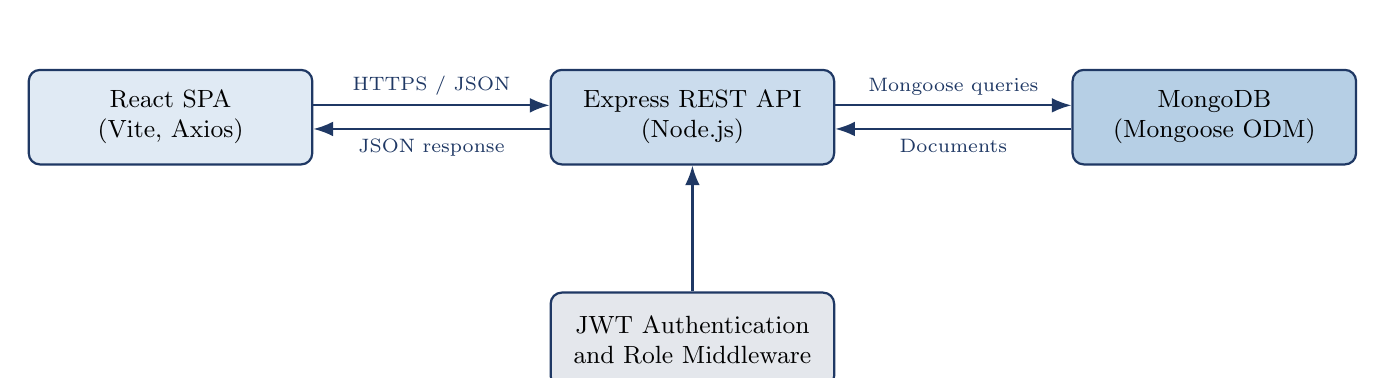
\begin{tikzpicture}[
  box/.style={rectangle, rounded corners, draw=primary, fill=lightgray, minimum width=3.6cm, minimum height=1.2cm, align=center, font=\small, line width=0.8pt},
  arr/.style={-{Latex[length=2.5mm]}, thick, primary}
]
\node[box, fill=accent!15] (client) {React SPA\\(Vite, Axios)};
\node[box, right=3cm of client, fill=accent!25] (api) {Express REST API\\(Node.js)};
\node[box, right=3cm of api, fill=accent!35] (db) {MongoDB\\(Mongoose ODM)};

\node[box, below=1.6cm of api, minimum width=3.6cm, fill=primary!12] (mw) {JWT Authentication\\and Role Middleware};

\draw[arr] ($(client.east)+(0,0.15)$) -- node[above, font=\scriptsize]{HTTPS / JSON} ($(api.west)+(0,0.15)$);
\draw[arr] ($(api.west)+(0,-0.15)$) -- node[below, font=\scriptsize]{JSON response} ($(client.east)+(0,-0.15)$);
\draw[arr] ($(api.east)+(0,0.15)$) -- node[above, font=\scriptsize]{Mongoose queries} ($(db.west)+(0,0.15)$);
\draw[arr] ($(db.west)+(0,-0.15)$) -- node[below, font=\scriptsize]{Documents} ($(api.east)+(0,-0.15)$);
\draw[arr] (mw) -- (api);
\end{tikzpicture}
\caption{Three-tier architecture of the Mentorship Management System}
\end{figure}

\section{Request Flow}
\sectionrule
Every protected request travels through the same pipeline before reaching business logic:

\begin{enumerate}[itemsep=2pt]
  \item The React client sends an HTTP request through Axios to an Express route. For protected endpoints, it attaches a JWT in the \texttt{Authorization: Bearer <token>} header. The token was issued at login and is stored on the client after authentication.
  \item The \texttt{protect} middleware reads the header, verifies the token's signature using the server's JWT secret, and, if valid, decodes the user's identity and role onto \texttt{req.user}. If the token is missing or invalid, the middleware short-circuits the request with a 401 response.
  \item The \texttt{authorizeRoles(...)} middleware checks that \texttt{req.user.role} is in the list of roles permitted for that route. For example, only a user with the \texttt{faculty} role may call the mentor-approval endpoint, and only \texttt{admin} may call the reassignment endpoint. A user with the wrong role receives a 403 response.
  \item The matching controller function executes the business logic for that operation, reading and writing data through the relevant Mongoose model or models.
  \item A JSON response with a \texttt{success} flag, a human-readable \texttt{message}, and, where applicable, a \texttt{data} payload is returned to the client.
\end{enumerate}

\section{Folder Structure}
\sectionrule
The backend and frontend are organized as two separate projects, connected only through the REST API contract. This separation allows the two halves to be developed, tested, and deployed independently.

\begin{lstlisting}[language=bash, caption={Backend folder structure}]
mentorship-backend/
  src/
    config/db.js            # MongoDB connection setup
    controllers/             # Business logic per resource
    middleware/               # Auth and error handling
    models/                   # Mongoose schemas
    routes/                    # Express routers per resource
    utils/asyncHandler.js
    server.js                 # Application entry point
\end{lstlisting}

\begin{lstlisting}[language=bash, caption={Frontend folder structure}]
mentorship-frontend/
  src/
    components/                # Navbar, Sidebar, Modal, StatCard, and others
    context/AuthContext.jsx    # Authentication state provider
    pages/
      admin/                    # AdminDashboard, DepartmentSummary, ReassignMentee
      faculty/                  # FacultyDashboard, Mentees, Availability, AddNote
      student/                  # StudentDashboard, RequestMentor, BookMeeting
      Login.jsx, Register.jsx
    services/api.js            # Configured Axios instance and API calls
\end{lstlisting}

% ================= CHAPTER 4: USE CASE ANALYSIS =================
\chapter{Use Case Analysis}

\section{Actors}
\sectionrule
The system has three primary actors, each mapped directly to the \texttt{role} field on the \texttt{User} model.

\begin{longtable}{@{}p{2.6cm}p{11cm}@{}}
\toprule
\textbf{Actor} & \textbf{Description} \\
\midrule
\endhead
Student & A registered student who can request a mentor, book meetings with their assigned mentor, view their meeting history, and submit feedback. \\
Faculty & A registered faculty member acting as a mentor. Can review and approve incoming mentor requests, manage availability, view assigned mentees, and add notes to meetings. \\
Admin & An administrative user with system-wide visibility. Can view department-level summaries and reassign a student from one mentor to another. \\
\bottomrule
\end{longtable}

\section{Use Case Diagram}
\sectionrule
Figure 4.1 groups each actor with the use cases specific to that role. All three roles authenticate through the same registration and login screen; this shared entry point is shown once, under the Student actor, and applies equally to Faculty and Admin.

\begin{figure}[h]
\centering
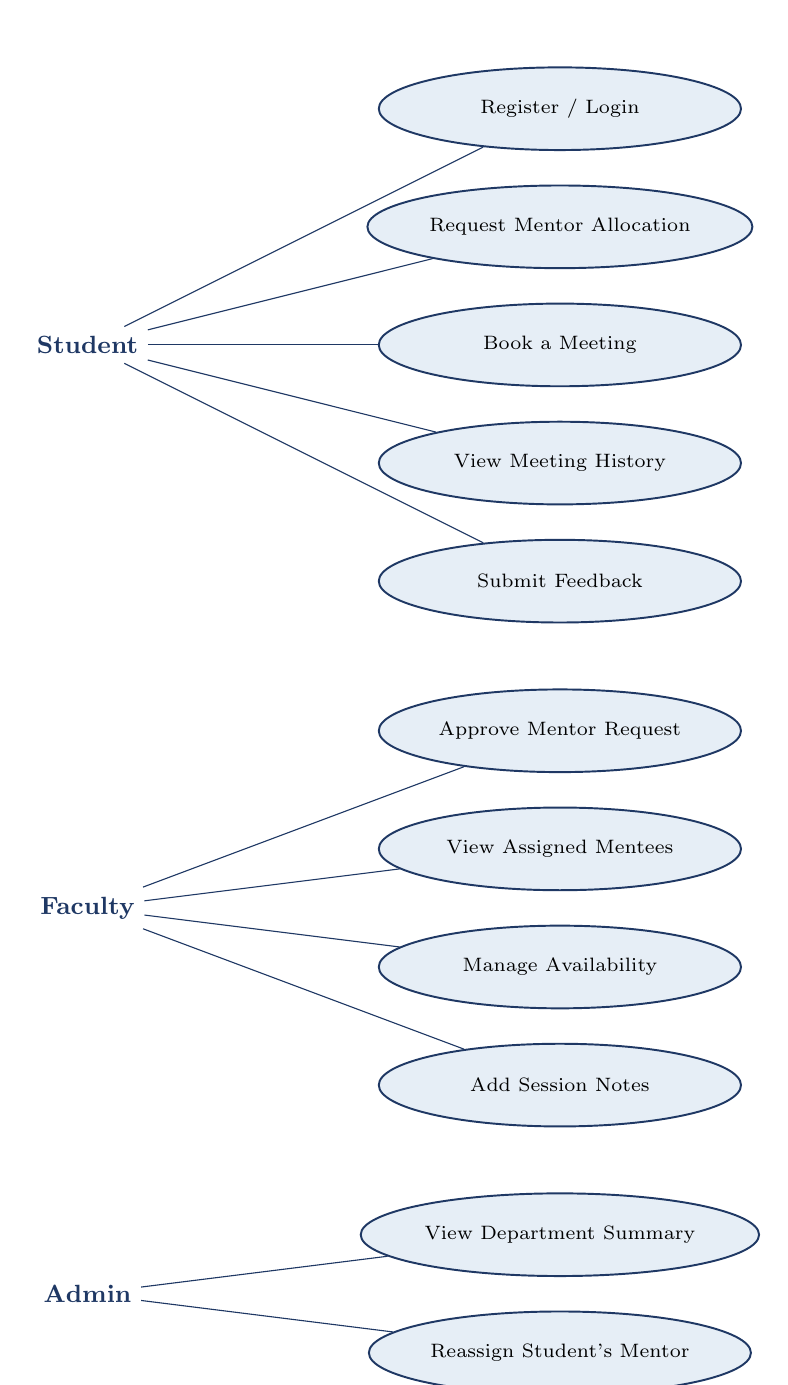
\begin{tikzpicture}[
  actor/.style={font=\small\bfseries, align=center, text=primary},
  usecase/.style={ellipse, draw=primary, fill=accent!12, minimum width=4.6cm, minimum height=1.05cm, align=center, font=\scriptsize, line width=0.7pt, inner sep=2pt},
  conn/.style={primary, thin}
]

% ---- Student band ----
\node[actor] (student) at (0,6.6) {Student};
\node[usecase] (uc1) at (6,9.6)  {Register / Login};
\node[usecase] (uc2) at (6,8.1)  {Request Mentor Allocation};
\node[usecase] (uc3) at (6,6.6)  {Book a Meeting};
\node[usecase] (uc4) at (6,5.1)  {View Meeting History};
\node[usecase] (uc5) at (6,3.6)  {Submit Feedback};

\draw[conn] (student) -- (uc1);
\draw[conn] (student) -- (uc2);
\draw[conn] (student) -- (uc3);
\draw[conn] (student) -- (uc4);
\draw[conn] (student) -- (uc5);

% ---- Faculty band ----
\node[actor] (faculty) at (0,-0.55) {Faculty};
\node[usecase] (uc6) at (6,1.7)  {Approve Mentor Request};
\node[usecase] (uc7) at (6,0.2)  {View Assigned Mentees};
\node[usecase] (uc8) at (6,-1.3) {Manage Availability};
\node[usecase] (uc9) at (6,-2.8) {Add Session Notes};

\draw[conn] (faculty) -- (uc6);
\draw[conn] (faculty) -- (uc7);
\draw[conn] (faculty) -- (uc8);
\draw[conn] (faculty) -- (uc9);

% ---- Admin band ----
\node[actor] (admin) at (0,-5.45) {Admin};
\node[usecase] (uc10) at (6,-4.7) {View Department Summary};
\node[usecase] (uc11) at (6,-6.2) {Reassign Student's Mentor};

\draw[conn] (admin) -- (uc10);
\draw[conn] (admin) -- (uc11);

\end{tikzpicture}
\caption{Use case diagram showing actor to use case relationships}
\end{figure}

\section{Use Case Descriptions}
\sectionrule
\textbf{UC: Request Mentor Allocation.} A student with no active mentor submits a request, optionally naming a preferred faculty member. The system rejects the request if the student already has a pending request. The request is stored as an \texttt{Assignment} document with status \texttt{pending}.

\textbf{UC: Approve Mentor Request.} A faculty member views all pending requests, then approves one. On approval, the assignment status changes to \texttt{active}, the faculty's identity is attached to the assignment, and the student's own \texttt{mentor} reference is updated to point at that faculty member's mentor profile.

\textbf{UC: Reassign Mentor.} An admin selects an existing assignment and specifies a new faculty member. The system verifies the target user exists and holds the \texttt{faculty} role, updates the assignment, sets its \texttt{reassignedFlag} to true, and updates the student's mentor reference to match.

\textbf{UC: Book Meeting.} A student with an active mentor schedules a meeting for a chosen date, with an optional agenda. The meeting starts in \texttt{scheduled} status and can later be marked \texttt{completed} or \texttt{cancelled}.

\textbf{UC: Submit Feedback.} After a meeting, a student submits a rating from 1 to 5 together with an optional free-text comment, tied to that specific meeting.

% ================= CHAPTER 5: DATABASE DESIGN =================
\chapter{Database Design}

\section{Entity Overview}
\sectionrule
The system uses seven core Mongoose collections. Relationships between them are expressed through \texttt{ObjectId} references rather than embedded documents, which keeps each collection independently queryable and avoids duplicating data such as user profiles across records.

\begin{longtable}{@{}p{2.6cm}p{11cm}@{}}
\toprule
\textbf{Model} & \textbf{Purpose and Key Fields} \\
\midrule
\endhead
\texttt{User} & The base account for every person in the system: name, email (unique), a bcrypt-hashed password, a role of \texttt{student}, \texttt{faculty}, or \texttt{admin}, and a department. All authentication is performed against this collection. \\
\texttt{Student} & Extends a User with a unique roll number, department, semester (1 to 12), and a reference to the currently assigned \texttt{Mentor}. \\
\texttt{Mentor} & Extends a User with department, a list of expertise tags, and a free-text availability field. \\
\texttt{Assignment} & The link between a student and a faculty mentor. Tracks a status of \texttt{pending}, \texttt{active}, \texttt{reassigned}, or \texttt{completed}, the date assigned, and a boolean \texttt{reassignedFlag} that records whether the student has been moved from their original mentor. \\
\texttt{Meeting} & A scheduled mentor and student meeting: date, an optional agenda, a status of \texttt{scheduled}, \texttt{completed}, or \texttt{cancelled}, and a notes field. \\
\texttt{Note} & A standalone note tied to a specific meeting through \texttt{meetingId}, used for more detailed session records than the meeting's own notes field. \\
\texttt{Feedback} & Student feedback tied to a specific meeting: a required rating from 1 to 5 and an optional comment. \\
\bottomrule
\end{longtable}

All seven schemas use Mongoose's \texttt{timestamps} option, so every document automatically records \texttt{createdAt} and \texttt{updatedAt}, which supports both the department summary statistics and general auditability.

\section{Entity Relationship Diagram}
\sectionrule
\begin{figure}[h]
\centering
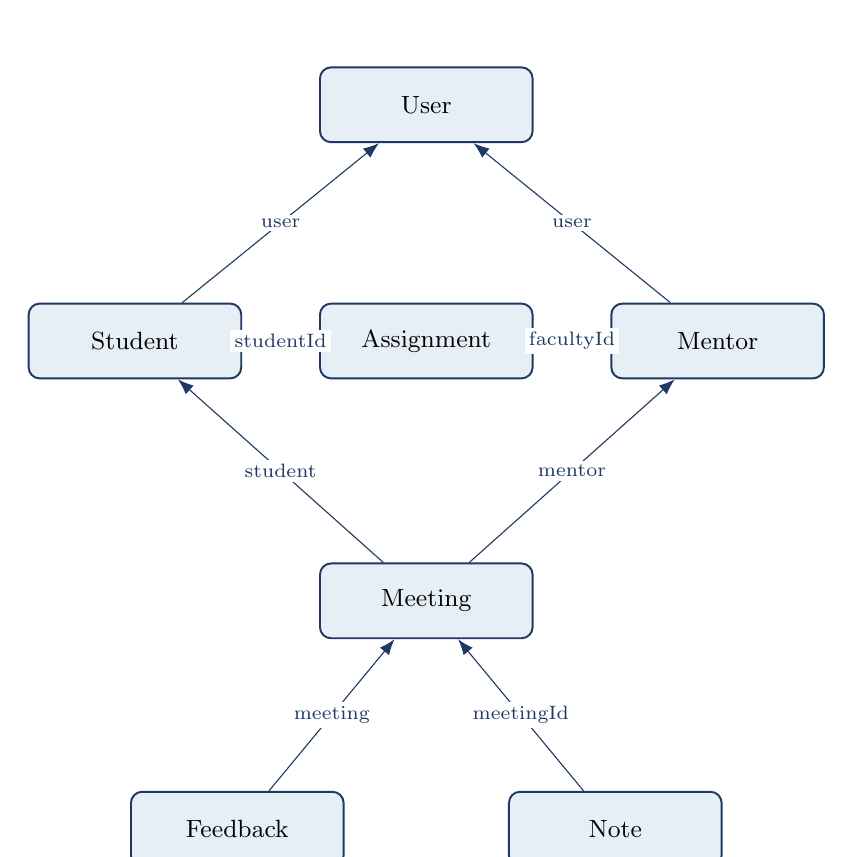
\begin{tikzpicture}[
  ent/.style={rectangle, draw=primary, fill=accent!12, rounded corners, minimum width=2.7cm, minimum height=0.95cm, font=\small, align=center, line width=0.7pt},
  rel/.style={-{Latex[length=2mm]}, primary, thin},
  lbl/.style={font=\scriptsize, fill=white, inner sep=1.5pt}
]
\node[ent] (user) at (5,10) {User};
\node[ent] (student) at (1.3,7) {Student};
\node[ent] (mentor) at (8.7,7) {Mentor};
\node[ent] (assignment) at (5,7) {Assignment};
\node[ent] (meeting) at (5,3.7) {Meeting};
\node[ent] (feedback) at (2.6,0.8) {Feedback};
\node[ent] (note) at (7.4,0.8) {Note};

\draw[rel] (student) -- node[lbl]{user} (user);
\draw[rel] (mentor) -- node[lbl]{user} (user);
\draw[rel] (assignment) -- node[lbl]{studentId} (student);
\draw[rel] (assignment) -- node[lbl]{facultyId} (mentor);
\draw[rel] (meeting) -- node[lbl]{student} (student);
\draw[rel] (meeting) -- node[lbl]{mentor} (mentor);
\draw[rel] (feedback) -- node[lbl]{meeting} (meeting);
\draw[rel] (note) -- node[lbl]{meetingId} (meeting);
\end{tikzpicture}
\caption{Entity relationship diagram of the seven core collections}
\end{figure}

\section{Relationship Notes}
\sectionrule
\begin{itemize}[itemsep=2pt]
  \item A \texttt{Student} and a \texttt{Mentor} document each reference exactly one underlying \texttt{User}, which keeps authentication data separate from role-specific profile data.
  \item An \texttt{Assignment} is the record of truth for who is currently mentoring whom, while the \texttt{Student.mentor} field is a denormalized pointer kept in sync whenever an assignment is approved or reassigned, so that mentor lookups for a student do not require querying the assignment collection first.
  \item A \texttt{Meeting} references both a \texttt{Mentor} and a \texttt{Student} directly, so meeting history can be queried from either side of the relationship.
  \item Both \texttt{Note} and \texttt{Feedback} attach to a \texttt{Meeting}. \texttt{Feedback} additionally stores its own direct \texttt{student} reference, so a student's feedback history can be queried without joining through \texttt{Meeting}.
\end{itemize}

% ================= CHAPTER 6: MODULES AND FEATURES =================
\chapter{Modules and Features}

\section{Authentication and User Management}
\sectionrule
Every user, regardless of role, is created and authenticated through the same \texttt{User} collection and the same pair of endpoints, \texttt{POST /api/users} for registration and \texttt{POST /api/users/login} for authentication. Passwords are hashed with \texttt{bcryptjs} before being stored, so the raw password is never persisted. On successful login, the server issues a signed JWT that encodes the user's identity and role. All subsequent protected requests present this token, which is verified by the \texttt{protect} middleware and checked against permitted roles by \texttt{authorizeRoles}.

\section{Student Module}
\sectionrule
The student dashboard is the entry point for a student's mentorship activity. From here a student can:
\begin{itemize}[itemsep=2pt]
  \item Submit a mentor allocation request, optionally naming a preferred faculty member.
  \item View their currently assigned mentor once a request has been approved.
  \item Book a meeting with their mentor, specifying a date and an agenda.
  \item Review their complete meeting history, including past, scheduled, and cancelled meetings.
  \item Submit feedback, a 1 to 5 rating and an optional comment, after a completed meeting.
\end{itemize}

\section{Faculty Module}
\sectionrule
Faculty members act as mentors and interact with the system primarily through the faculty dashboard:
\begin{itemize}[itemsep=2pt]
  \item Review a list of pending mentor allocation requests addressed to them or open generally.
  \item Approve a request, which activates the assignment and updates the student's mentor reference.
  \item View a list of currently assigned mentees.
  \item Update their own availability so students can see when they are reachable.
  \item View and manage upcoming meetings, and add structured notes to a completed session.
\end{itemize}

\section{Admin Module}
\sectionrule
The admin dashboard gives an institution-wide view of mentorship activity:
\begin{itemize}[itemsep=2pt]
  \item A department-wise summary showing total students, total faculty, total and active assignments, reassigned students, and meeting counts broken down by status.
  \item The ability to reassign a student from one mentor to another, which is used when a faculty member becomes unavailable or a mismatch needs correcting.
\end{itemize}

\section{Meetings, Notes, and Feedback}
\sectionrule
Meetings are the operational core of the system once a mentor is assigned:
\begin{itemize}[itemsep=2pt]
  \item Meetings can be created, listed, have their notes updated, and be cancelled.
  \item Additional structured notes can be attached to a specific meeting through the notes module, independent of the meeting's own notes field, which allows multiple contributors to record observations over time.
  \item Feedback is collected once a meeting has taken place, giving the system a simple but effective quality signal per mentor and per department.
\end{itemize}

% ================= CHAPTER 7: SEQUENCE DIAGRAMS =================
\chapter{Sequence Diagrams}

\section{User Login}
\sectionrule
\begin{figure}[h]
\centering
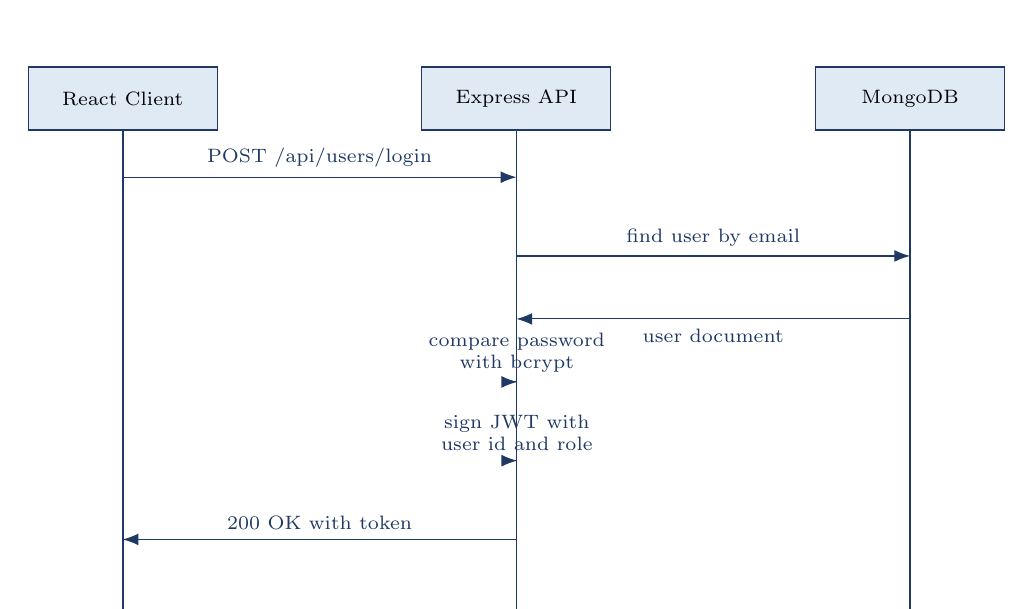
\begin{tikzpicture}[
  life/.style={draw=primary, line width=0.6pt},
  actorbox/.style={rectangle, draw=primary, fill=accent!15, minimum width=2.4cm, minimum height=0.8cm, align=center, font=\scriptsize},
  msg/.style={-{Latex[length=2mm]}, primary, font=\scriptsize}
]
\node[actorbox] (c) at (0,0) {React Client};
\node[actorbox] (a) at (5,0) {Express API};
\node[actorbox] (d) at (10,0) {MongoDB};

\draw[life] (c.south) -- ++(0,-6.2);
\draw[life] (a.south) -- ++(0,-6.2);
\draw[life] (d.south) -- ++(0,-6.2);

\draw[msg] (0,-1) -- node[above]{POST /api/users/login} (5,-1);
\draw[msg] (5,-2) -- node[above]{find user by email} (10,-2);
\draw[msg] (10,-2.8) -- node[below]{user document} (5,-2.8);
\draw[msg] (5,-3.6) -- node[above, align=center]{compare password\\with bcrypt} (5.01,-3.6);
\draw[msg] (5,-4.6) -- node[above, align=center]{sign JWT with\\user id and role} (5.01,-4.6);
\draw[msg] (5,-5.6) -- node[above]{200 OK with token} (0,-5.6);
\end{tikzpicture}
\caption{Sequence diagram for user login and JWT issuance}
\end{figure}

\section{Mentor Request and Approval}
\sectionrule
\begin{figure}[h]
\centering
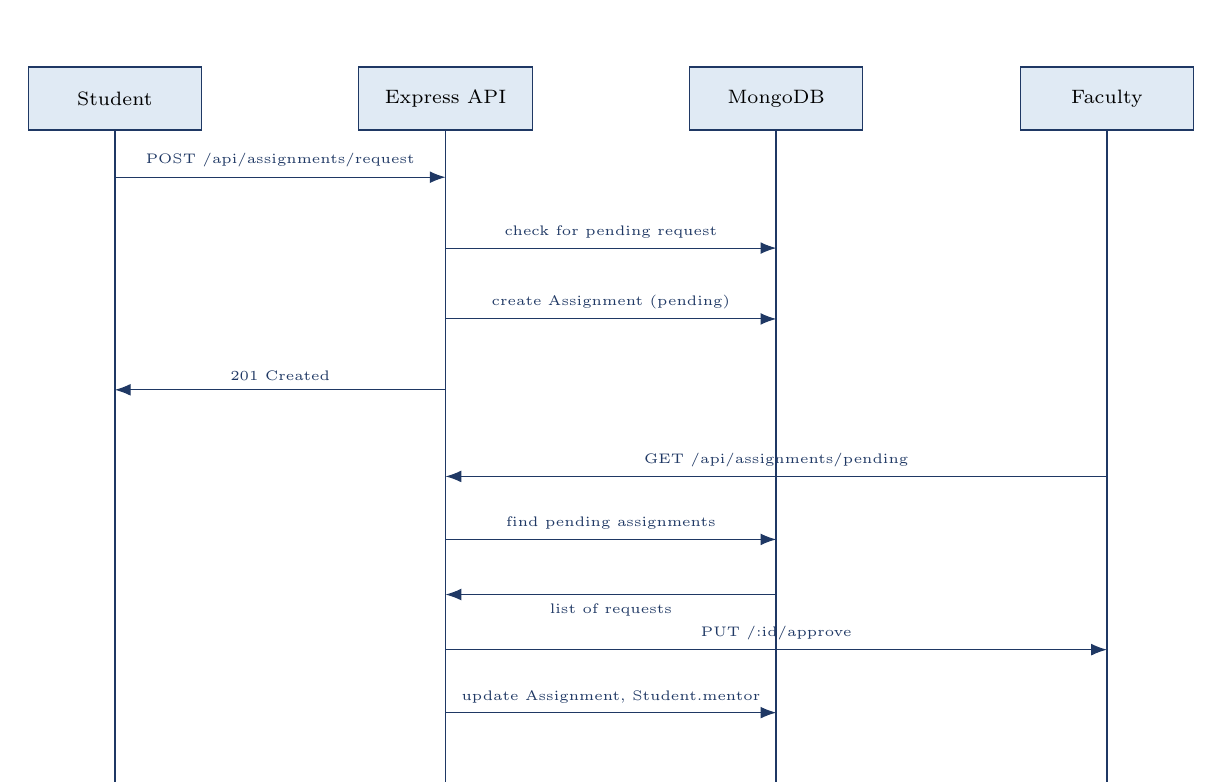
\begin{tikzpicture}[
  life/.style={draw=primary, line width=0.6pt},
  actorbox/.style={rectangle, draw=primary, fill=accent!15, minimum width=2.2cm, minimum height=0.8cm, align=center, font=\scriptsize},
  msg/.style={-{Latex[length=2mm]}, primary, font=\scriptsize}
]
\node[actorbox] (s) at (0,0)  {Student};
\node[actorbox] (a) at (4.2,0)  {Express API};
\node[actorbox] (db) at (8.4,0) {MongoDB};
\node[actorbox] (f) at (12.6,0) {Faculty};

\draw[life] (s.south) -- ++(0,-8.4);
\draw[life] (a.south) -- ++(0,-8.4);
\draw[life] (db.south) -- ++(0,-8.4);
\draw[life] (f.south) -- ++(0,-8.4);

\draw[msg] (0,-1) -- node[above, align=center, font=\tiny]{POST /api/assignments/request} (4.2,-1);
\draw[msg] (4.2,-1.9) -- node[above, font=\tiny]{check for pending request} (8.4,-1.9);
\draw[msg] (4.2,-2.8) -- node[above, font=\tiny]{create Assignment (pending)} (8.4,-2.8);
\draw[msg] (4.2,-3.7) -- node[above, font=\tiny]{201 Created} (0,-3.7);

\draw[msg] (12.6,-4.8) -- node[above, font=\tiny]{GET /api/assignments/pending} (4.2,-4.8);
\draw[msg] (4.2,-5.6) -- node[above, font=\tiny]{find pending assignments} (8.4,-5.6);
\draw[msg] (8.4,-6.3) -- node[below, font=\tiny]{list of requests} (4.2,-6.3);
\draw[msg] (4.2,-7.0) -- node[above, font=\tiny]{PUT /:id/approve} (12.6,-7.0);
\draw[msg] (4.2,-7.8) -- node[above, font=\tiny]{update Assignment, Student.mentor} (8.4,-7.8);
\end{tikzpicture}
\caption{Sequence diagram for the mentor request and approval workflow}
\end{figure}

\section{Meeting and Feedback}
\sectionrule
\begin{figure}[h]
\centering
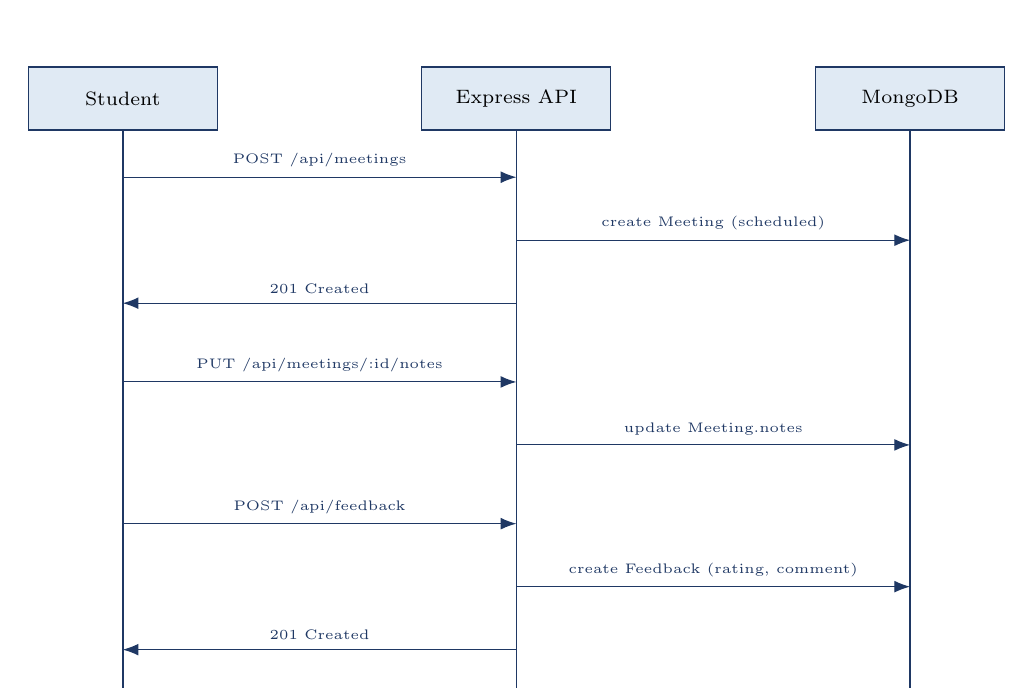
\begin{tikzpicture}[
  life/.style={draw=primary, line width=0.6pt},
  actorbox/.style={rectangle, draw=primary, fill=accent!15, minimum width=2.4cm, minimum height=0.8cm, align=center, font=\scriptsize},
  msg/.style={-{Latex[length=2mm]}, primary, font=\scriptsize}
]
\node[actorbox] (s) at (0,0) {Student};
\node[actorbox] (a) at (5,0) {Express API};
\node[actorbox] (d) at (10,0) {MongoDB};

\draw[life] (s.south) -- ++(0,-7.2);
\draw[life] (a.south) -- ++(0,-7.2);
\draw[life] (d.south) -- ++(0,-7.2);

\draw[msg] (0,-1) -- node[above, font=\tiny]{POST /api/meetings} (5,-1);
\draw[msg] (5,-1.8) -- node[above, font=\tiny]{create Meeting (scheduled)} (10,-1.8);
\draw[msg] (5,-2.6) -- node[above, font=\tiny]{201 Created} (0,-2.6);
\draw[msg] (0,-3.6) -- node[above, font=\tiny]{PUT /api/meetings/:id/notes} (5,-3.6);
\draw[msg] (5,-4.4) -- node[above, font=\tiny]{update Meeting.notes} (10,-4.4);
\draw[msg] (0,-5.4) -- node[above, font=\tiny]{POST /api/feedback} (5,-5.4);
\draw[msg] (5,-6.2) -- node[above, font=\tiny]{create Feedback (rating, comment)} (10,-6.2);
\draw[msg] (5,-7.0) -- node[above, font=\tiny]{201 Created} (0,-7.0);
\end{tikzpicture}
\caption{Sequence diagram for booking a meeting and submitting feedback}
\end{figure}

% ================= CHAPTER 8: API REFERENCE =================
\chapter{API Reference}

\section{Conventions}
\sectionrule
All endpoints are prefixed with \texttt{/api}. Protected routes require an \texttt{Authorization: Bearer <token>} header carrying a valid JWT. Every response follows the shape \texttt{\{ success, message, data \}}, where \texttt{data} is omitted for simple confirmations.

\section{Endpoint Summary}
\sectionrule
\begin{longtable}{@{}p{1.3cm}p{5.2cm}p{2.1cm}p{4.3cm}@{}}
\toprule
\textbf{Method} & \textbf{Endpoint} & \textbf{Access} & \textbf{Description} \\
\midrule
\endhead
GET & \url{/api/health} & Public & API health check \\
POST & \url{/api/users} & Public & Register a new user \\
POST & \url{/api/users/login} & Public & Log in, receive a JWT \\
GET & \url{/api/users} & Public & List users \\
POST & \url{/api/mentors} & Public & Create a mentor profile \\
GET & \url{/api/mentors} & Public & List mentors \\
GET & \url{/api/mentors/:id/mentees} & Public & List a mentor's mentees \\
PUT & \url{/api/mentors/:id/availability} & Public & Update mentor availability \\
POST & \url{/api/students} & Public & Create a student profile \\
GET & \url{/api/students} & Public & List students \\
GET & \url{/api/students/:id/mentor} & Public & Get a student's assigned mentor \\
GET & \url{/api/students/:id/meetings} & Public & Get a student's meetings \\
POST & \url{/api/assignments} & Public & Create an assignment directly \\
GET & \url{/api/assignments} & Public & List assignments \\
GET & \url{/api/assignments/summary} & Public & Department-wise summary \\
POST & \url{/api/assignments/request} & Student & Request mentor allocation \\
GET & \url{/api/assignments/pending} & Faculty & View pending requests \\
PUT & \url{/api/assignments/:id/approve} & Faculty & Approve a mentor request \\
PUT & \url{/api/assignments/:id/reassign} & Admin & Reassign a student's mentor \\
POST & \url{/api/meetings} & Public & Schedule a meeting \\
GET & \url{/api/meetings} & Public & List meetings \\
PUT & \url{/api/meetings/:id/notes} & Public & Update meeting notes \\
PUT & \url{/api/meetings/:id/cancel} & Public & Cancel a meeting \\
POST & \url{/api/notes} & Public & Create a note \\
GET & \url{/api/notes} & Public & List notes \\
GET & \url{/api/notes/meeting/:meetingId} & Public & Notes for a specific meeting \\
POST & \url{/api/feedback} & Public & Submit feedback \\
GET & \url{/api/feedback} & Public & List feedback \\
\bottomrule
\end{longtable}

\textit{Note: ``Public'' here means the route is not currently wrapped in the \texttt{protect} middleware in this version of the codebase. Role-gated routes, marked Student, Faculty, or Admin, are enforced with \texttt{protect} together with \texttt{authorizeRoles}.}

\section{Sample Request and Response}
\sectionrule
The listing below shows the request body and response shape for approving a mentor request, taken directly from the assignment controller.

\begin{lstlisting}[language=bash, caption={Request}]
PUT /api/assignments/68f2c1.../approve
Authorization: Bearer <faculty JWT>
\end{lstlisting}

\begin{lstlisting}[caption={Response}]
{
  "success": true,
  "message": "Mentor request approved successfully",
  "data": {
    "_id": "68f2c1...",
    "studentId": { "...": "populated student" },
    "facultyId": { "...": "populated faculty" },
    "status": "active",
    "reassignedFlag": false
  }
}
\end{lstlisting}

% ================= CHAPTER 9: SECURITY =================
\chapter{Security Considerations}

\section{Implemented}
\sectionrule
\begin{itemize}[itemsep=2pt]
  \item Password hashing through \texttt{bcryptjs}, so plaintext passwords are never stored in the database.
  \item Stateless authentication using signed JWTs, verified independently on every protected request.
  \item Role-based access control on the sensitive assignment operations: a student may request a mentor, only faculty may approve requests, and only an admin may reassign a student.
  \item CORS enabled at the API boundary for controlled cross-origin access from the frontend.
\end{itemize}

\section{Recommended Hardening}
\sectionrule
The following items are recommended as future hardening steps before any production deployment:
\begin{itemize}[itemsep=2pt]
  \item Apply the \texttt{protect} and \texttt{authorizeRoles} middleware consistently across all remaining routes; several list and create endpoints are currently open, as noted in the API reference.
  \item Route every controller's error handling through the centralized \texttt{errorMiddleware} for consistent, predictable error responses.
  \item Add request body validation, for example with \texttt{express-validator} or \texttt{zod}, on all POST and PUT endpoints.
  \item Remove secrets entirely from source control and rotate the JWT signing secret on a regular schedule.
  \item Add rate limiting on the login endpoint to reduce the risk of brute-force credential attacks.
\end{itemize}

% ================= CHAPTER 10: TESTING =================
\chapter{Testing}

\section{Approach}
\sectionrule
Testing during development was carried out primarily at the API level, using Postman as the client. The backend repository includes a dedicated \texttt{postman} directory containing exported resources and workspace globals, which were used to exercise every endpoint against a running instance of the API and a MongoDB Atlas development database.

\section{What Was Tested}
\sectionrule
\begin{itemize}[itemsep=2pt]
  \item Registration and login, including rejection of duplicate emails and incorrect passwords.
  \item Token verification, confirming that requests without a valid \texttt{Authorization} header are rejected with a 401 response.
  \item Role enforcement, confirming that a student token cannot call the faculty approval endpoint and that a faculty token cannot call the admin reassignment endpoint.
  \item The full mentor request and approval life cycle, from a student's initial request through to an active assignment and an updated \texttt{Student.mentor} reference.
  \item Meeting creation, note updates, and cancellation, including the effect on subsequent meeting listings.
  \item Feedback submission and its constraint that the rating must fall between 1 and 5.
  \item The department summary endpoint, cross-checked manually against known seed data to confirm the returned counts were correct.
\end{itemize}

\section{Manual Frontend Verification}
\sectionrule
Each role's dashboard was manually walked through end to end: registering as a student, requesting a mentor, logging in as faculty to approve the request, booking and completing a meeting, submitting feedback, and finally logging in as an admin to confirm the department summary reflected the activity performed.

% ================= CHAPTER 11: CONCLUSION =================
\chapter{Conclusion and Future Scope}

\section{Current Status}
\sectionrule
The project delivers a working, end-to-end mentorship platform. A student can register, request a mentor, have that request approved by faculty, book and manage meetings, and leave feedback, while an admin retains full oversight through department summaries and reassignment controls. The backend exposes a complete REST API across seven resource domains, secured with JWT authentication and role-based authorization on all sensitive operations, and the frontend provides distinct, role-appropriate dashboards for all three user types.

\section{Key Outcomes}
\sectionrule
\begin{itemize}[itemsep=2pt]
  \item A clean separation between authentication identity (\texttt{User}) and role-specific profile data (\texttt{Student}, \texttt{Mentor}), which keeps the schema easy to extend.
  \item A complete mentor allocation workflow, from request through approval to reassignment, modeled explicitly as an \texttt{Assignment} state machine.
  \item A meeting and feedback subsystem that gives the institution a lightweight but genuine quality signal on mentorship activity.
  \item A frontend built around role-specific dashboards rather than a single generic interface, which keeps each user's experience focused on the actions relevant to them.
\end{itemize}

\section{Future Scope}
\sectionrule
\begin{itemize}[itemsep=2pt]
  \item Email or in-app notifications for meeting scheduling and mentor request approval.
  \item Calendar integration for mentor availability and meeting booking.
  \item An analytics dashboard for admins, covering meeting frequency and feedback trends over time.
  \item File or document attachment support for meeting notes.
  \item A deployment pipeline with CI/CD and containerization to move the prototype toward production readiness.
  \item Completing the security hardening items listed in Chapter 9 before any real-world rollout.
\end{itemize}

\end{document}
